The evaluation is concerned with feasibility of the motion model, as well as
it two primary objectives; Web availability and simplicity for developers.


\subsection {Motion Synchronization}

The research group has used motion synchronization for a wide range of
technical demonstration since 2010. An early evaluation of the research
prototype is discussed in the paper titled \emph{The Media State
Vector}~\cite{msv}. Though the interpretations of the experiments are
conservative, the key findings indicate that motion synchronization can
provide frame rate levels of accuracy (33 milliseconds). With the introduction
of WebSockets in the InMotion service, results have improved significantly.
Synchronization errors are in the order of a few milliseconds on all major
browsers and most operating systems (including Android).


Sect.~\ref{sec:motionsync} discussed motion synchronization, and reported
synchronizations errors in the 0-5 millisecond range. Typically we observe 0-1
millisecond errors for desktop browsers, compared to a system clock
synchronized by NTS. These results are achieved using the \emph{InMotion}
service provided by Motion Corporation~\cite{mcorp}. This service has been running
continuously for years, supporting a wide range of technical demonstrations,
at any time, at any place, and across a wide range of devices. As such, the
value of a production grade service is also confirmed.



\runinhead{Future improvements:}

Though the accuracy of online clock synchronization is acceptable for a wide
range of applications, improvements are always attractive. One proposal could
be to leverage the availability of synchronized system clocks. NTP~\cite{ntp}
and PTP~\cite{ptp} are widely used and trusted protocols for large-scale,
precise clock synchronization. Unfortunately, at present this is not possible.
Synchronized system clocks is not a safe assumption in the Web domain, and Web
clients do not expose any information indicating the quality of
synchronization that can be expected from a systems clock. However, if this
changes in the future, implementations of motion synchronization may take
advantage of this.

Alternatively, one might imagine a cloud hosted clock service growing more
similar to NTP and PTP. For instance, it would be possible to reduce latency
for clients by decentralizing the service. Synchronizing clients would then be
routed to a nearby server, measured by network latency. Such a decentralized
architecture would make the clock service more similar to NTP or PTP, though
it would be designed with different assumptions for access pattern and load.
PTP would be useful for clock synchronization internally in such a cloud-
hosted clock service.






\subsection {Synchronization of HTML media elements}



Sect.~\ref{sec:compsync} discussed synchronization of HTML5 media
elements, 

Two technical reports~\cite{syncreport1,syncreport2} document the abilities and
limitations of HTML5 media elements with respect to media synchronization, as
well the quality of synchronization achieved by the MediaSync library. In
short, for desktops, laptops and high-end smartphones, echoless audio playback
is expected both for video+audio and audio only. Smartphones, and embedded
devices such a ChromeCast, can be expected to provide frame accurate
synchronization. Target precision is generally achieved within 3 seconds. It
is also worth noting that measured results are consistent with human
observation. Echoless synchronization with the MediaSync library produces
various audio effects, like failing to hear one audio source, until volume
levels are changed and only the other audio source can be heard. Since these
effects are also achieved across browser types and architectures, this is a
strong indication that currentTime approximates the reference point
quite well (see Sect.~\ref{sec:referencepoint}).

\begin{figure}[h]
%\sidecaption
\centering
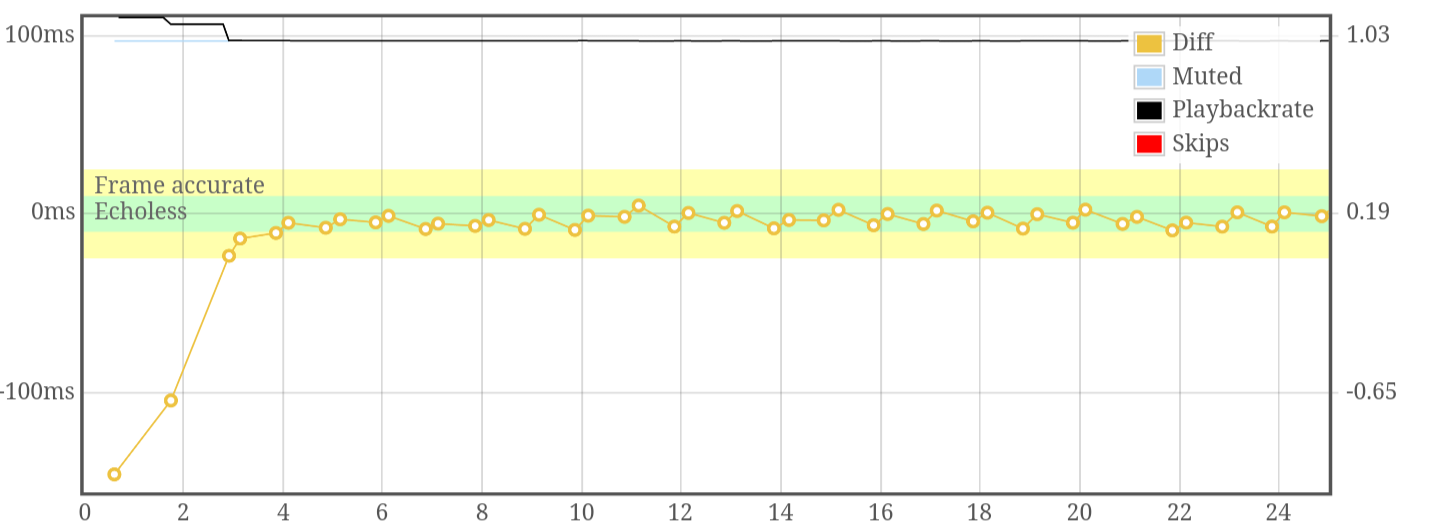
\includegraphics[scale=.23]{fig/android-video.png}
\caption{The figure illustrates an experiment with video (mp4) synchronization on
Android using Chrome browser. The plot shows currentTime compared to the ideal
playback position defined by motion. The green band (echoless) is +-10 millisecond and
the yellow (frame accurate is) +-25 millisecond. The media element enters frame accurate
playback after two seekTo operations, and converges on echoless using
variablePlaybackrate.}
\label{fig:videosync}
\end{figure}

Though echoless synchronization is generally achievable, there are always a
few combinations of architecture, browser and media format that pose problems.
Errors may also occur and vanish across software updates. To be able to
support echoless synchronization reliably across the board, standards must
include requirements for synchronization, and testing-suites must be developed
to ensure that those requirements are met. Ideally though, media
synchronization should be implemented natively in media elements. Given the
challenges faced by the MediaSync library, it is not unlikely that native
implementations would provide a significant improvement.




and reported how the MediaSync library produces synchronization
errors of about 7 milliseconds for both audio and video, as documented in
technical reports~\cite{syncreport1,syncreport2}. These results have been consistently
confirmed by day to day usage over several years. The user experience of
multi-device video synchronization is very good, to the point that errors are
hardly visible. The exception might be content with particular geometries and
rapid movements, as demonstrated by this video~\cite{carneval}. Synchronization
has also been maintained for hours and days at end, without any visible
errors. In addition, loading speeds are acceptable. Even though the MediaSync
library requires about 3 seconds to reach echoless, the experience is
perceived as acceptable much before this. A variety of video demonstrations
have been published at the Multi-device Timing Community Group
Website~\cite{mtcg}.


\subsection {Summary}


%this is good enough to
%support even the toughest challenge in Web-based media; echoless audio
%synchronization with HTML media elements. Furthermore, the accuracy of motion
%synchronization degrades well with poor network conditions. For instance,
%experiments with video synchronization in EDGE connectivity has not been
%visibly worse, except for longer update latency. In this instance, video data
%was fetched from local files. Conferences are also notorious hotspots for bad
%connectivity. In these circumstances, availability of media data consistently
%fails before synchronization.


Interestingly, the results for motion synchronization and HTML5 media
synchronization are well aligned with current limitations of the Web platform.
For instance, the precision of timed operation in JavaScript is about 1
millisecond, and a 60Hz screen refresh rate corresponds to 16 milliseconds.
Furthermore, these results also match limitations in human sensitivity to
synchronization errors. Identical audio signals skewed by less than 7
milliseconds will likely be interpreted as natural echo by the brain, and
collapsed into one signal (with directional information)~\cite{syncreport2}.

Finally, programming synchronized media experiences in the motion model is
both easy and rewarding. In our experience, motions and sequencers are
effective thinking tools as well as programming tools. A globally synchronized
video experience essentially requires three code statements.

With this, we argue that the feasibility of the motion model is confirmed. Web
availability for media synchronization is demonstrated by the \emph{InMotion} hosting
service for online motions. It is also clear that synchronization errors in
online synchronization are currently dominated by errors in synchronization in
HTML5 media elements. Future standardization efforts and optimizations would
likely yield significant improvements.




